\documentclass{article}
\usepackage[utf8]{inputenc} % Permite el uso de caracteres del Español
\usepackage[T1]{fontenc}
\usepackage{hyperref}
\usepackage{graphicx}
\usepackage{wrapfig}
\usepackage{subcaption}

% Para ecuaciones
\usepackage{amssymb, amsmath, amsbsy} % simbolitos
\usepackage{upgreek} % para poner letras griegas sin cursiva
\usepackage{cancel} % para tachar
\usepackage{mathdots} % para el comando \iddots
\usepackage{mathrsfs} % para formato de letra
\usepackage{stackrel} % para el comando \stackbin

% set font encoding for PDFLaTeX, XeLaTeX, or LuaTeX
\usepackage{ifxetex,ifluatex}
\newif\ifxetexorluatex
\ifxetex
  \xetexorluatextrue
\else
  \ifluatex
    \xetexorluatextrue
  \else
    \xetexorluatexfalse
  \fi
\fi

\ifxetexorluatex
  \usepackage{fontspec}
\else
  \usepackage[T1]{fontenc}
  \usepackage[utf8]{inputenc}
  \usepackage{lmodern}
\fi

\usepackage{hyperref}

\title{Actividad 10: \\ Teoría del Caos y el Mapeo Logístico}
\author{Melissa Matrecitos Avila}
\date{16 de mayo de 2018}

% Enable SageTeX to run SageMath code right inside this LaTeX file.
% http://mirrors.ctan.org/macros/latex/contrib/sagetex/sagetexpackage.pdf
% \usepackage{sagetex}

\begin{document}
\maketitle

\section{Introducción}
El siguiente reporte corresponde a la actividad 10 del curso de Física Computacional 1, en la cual se pide hacer una síntesis del artículo de Mapeo Logístico del blog de Geoff Boeing, pero en lugar de utilizar Python (haciendo uso del paquete pynamical) para realizar las imágenes, se utilizara wxMaxima.

El mapeo logístico es una aplicación matemática que se hizo muy conocida en 1976 gracias a un artículo científico del biólogo Robert May y que fue estudiada más en profundidad por el físico Mitchell Feigenbaum. May pretendía hallar un modelo demográfico sencillo que explicase la dinámica de una población de la que se ha supuesto que tiene un crecimiento cada vez más lento a medida que se acerca a una cantidad de individuos considerada como límite.Este modelo es a menudo citado como un ejemplo de representación de lo complejo que puede ser un comportamiento caótico aunque se parta de un modelo de sencilla expresió

El mapeo logístico puede expresarse matemáticamente como:

\begin{center}
$x_{n+1}=rx_{n}(1-x_{n})$
\end{center}

Donde:

$ x_{n} $ es un número entre cero y uno que representa a la fracción de individuos en un territorio, respecto de un $n^0$ supuesto máximo posible, en un instante "n".

$r$ es un número positivo que representa la relación o tasa combinada entre la reproducción y la mortandad.

Esta ecuación no lineal describe dos efectos:
\begin{itemize}
\item El crecimiento de tipo exponencial de la población.
\item La mortalidad adicional que aumenta a medida que crece la población, debido a la competencia de los individuos entre sí para asegurarse el alimento necesario.
\end{itemize}

EL reporte presenta una pequeña introducción al resumen, así como las secciones del blog y las imagénes correspondientes. Por último se presenta la sección de conclusión.

\section{Resumen}

La teoría del caos es una rama de las matemáticas que se ocupa de los sistemas dinámicos no lineales. Para enetender esto, es necesario saber qué es:
\begin{itemize}
\item Un sistema es un conjunto de componentes interactivos que forman un todo más grande. 
\item No lineal significa que el todo se convierte en algo más que simplemente sumar las partes individuales.
\item Dinámico significa que el sistema cambia con el tiempo en función de su estado actual.
\end{itemize}
Los sistemas caóticos son un subtipo simple de sistemas dinámicos no lineales, los cuales tienen una dependencia muy sensible de sus condiciones iniciales. Además, con el tiempo estos sistemas pueden producir un comportamiento totalmente impredecible y divergente (también conocido como caótico).

\subsection{El mapeo logístico}
Este modelo se basa en la función logística común de curva en forma de S que muestra cómo una población crece lentamente, luego rápidamente, antes de disminuir a medida que alcanza su capacidad de carga. El mapa de logística utiliza una ecuación de diferencia no lineal para observar los pasos de tiempo discretos. Se llama mapa logístico porque asigna el valor de la población en cualquier paso de tiempo a su valor en el siguiente paso:

\begin{center}
$x_{t+1}=rx_{t}(1-x_{t})$
\end{center}

Esta ecuación define las reglas o dinámicas de nuestro sistema: x representa la población en cualquier momento dado t, y r representa la tasa de crecimiento. En otras palabras, el nivel de población en cualquier momento dado es una función del parámetro de tasa de crecimiento y el nivel de población del paso de tiempo anterior. Si la tasa de crecimiento es demasiado baja, la población morirá y se extinguirá. Mayores tasas de crecimiento podrían establecerse hacia un valor estable o fluctuar a través de una serie de auges y caídas de la población.

\subsection{Comportamiento del sistema y atractores}

Para analizar el comportamiento de los sistemas, es conveniente hacer una gráfica de  Población vs Generación, permitiendo ver de manera sencilla como cambia la población conforme pasa el tiempo según sus tasas de crecimiento:

\begin{center}
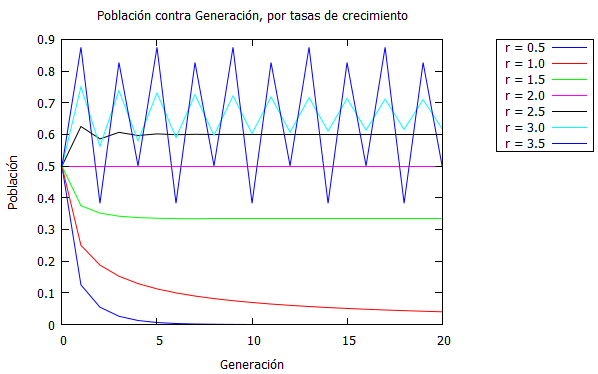
\includegraphics[width=.8\textwidth]{Imagen1.PNG}
\end{center}

Se puede ver que para la tasa de crecimiento 1.5,  el nivel de población se establece en un valor final de 0.33 después de algunas generaciones. Mientras que la tasa de crecimiento 2.0, tendrá un nivel de población constante en cada generación, representado una tasa de reemplazo. También se puede ver fácilmente como la tasa de crecimiento de 0.5 llega rápidamente al cero. Mientras que la línea correspondiente a una tasa de crecimiento para 3.0 parece estar convergiendo lentamente hacia un valor estable, la línea para 3.5 solo parece rebotar.


Un atractor es el valor, o conjunto de valores, con los que el sistema se establece a lo largo del tiempo. Dependiend del valor del parámetro de la tasa de creciemiento, este recibe un nombre, por ejemplo:

\begin{itemize}
\item \textbf{Atractor de punto fijo:} se da cuando el parámetro de tasa de crecimiento se establece en 0.5,es decir, el valor de la población se dibuja hacia 0 a lo largo del tiempo a medida que el modelo itera (línea azul).
\item \textbf{Ciclo límite:} Cuando el parámetro de tasa de crecimiento se establece en 3.5, el sistema oscila entre cuatro valores, como se muestra en la línea gris.
\item \textbf{Atractor extraño:} se da cuando ajustamos el parámetro de la tasa de crecimiento más allá de 3.5. Un sistema caótico tiene un atractor extraño, alrededor del cual el sistema oscila para siempre, nunca se repite o se establece en un estado estable de comportamiento. 
\end{itemize}

\subsection{Bifurcaciones y el Camino al Caos}

Un diagrama de bifurcación se utiliza cuando se tienen muchas tasas de crecimiento, por ejemplo, en la sección anterior, en vez de que tuviera 7 tasas, tener 1000. Este diagrama permite una visualización muy diferente:

\begin{center}
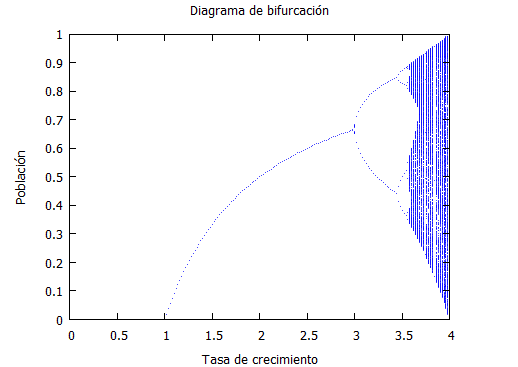
\includegraphics[width=.6\textwidth]{Imagen2.PNG}
\end{center}

Este diagrama se puede entender como 1000 segmentos verticales que corresponden a cada uno de los 1000 valores de las tasas de crecimiento. Arrojando los valores a los que que se dirige el mapa logístico para ese valor de parámetro, es decir, la porción vertical sobre cada tasa de crecimiento es el atractor de la tasa de crecimiento.

Analizando la imagen, se observa como las tasas de crecimiento entre 0 y 1 llevan a la extinción de la población. Para valores entre 1.0 y 3.0, el sistema siempre se establece en un nivel de población exacto y estable. Pero para algunas tasas de crecimiento, como 3.9, el diagrama muestra 100 valores diferentes, en otras palabras, un valor diferente para cada una de sus 100 generaciones. Nunca se establece en un punto fijo o un ciclo límite.

Para saber por qué se le da el nombre de diagrama de bifurcación, se analizará la gráfica en las tasas de crecimiento entre 2.8 y 4:

\begin{center}
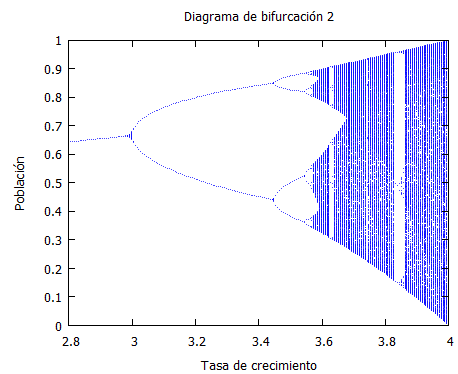
\includegraphics[width=.7\textwidth]{Imagen3.PNG}
\end{center}

Se puede observar que para la tasa de crecimiento de 3.0, los valores de la población se "bifurcan" en dos caminos, lo que quiere decir que a esa tasa de crecimiento, al aplicar la ecuación logística a uno de estos valores produce el otro. Siguiendo con el análisis, para el valor de 3.4, el diagrama se vuelve a bifurcar, hay cuatro caminos, en otras palabras, el sistema oscila más de cuatro valores de población, Para la tasa de crecimiento 3.5, se bifurca nuevamente en ocho caminos. Aquí, el sistema oscila más de ocho valores de población.

\subsection{El comienzo del caos}

Conforme la tasa de crecimiento crece, su mapa logístico comienza a oscilar en dos valores, después cuatro, ocho, diéciseis y treinta y dos valores de población. Estos son conocimos como periodos. Entonces al aumentar la tasa de crecimiento desde un valor de 3.6, las bifurcaciones aumentan hasta que el sistema es puede tomar cualquier valor de población. Esto se conoce como la manera que duplica el período al caos.

Para la tasa de crecimiento 3.9, la población se ha bifurcado tantas veces que el sistema ahora salta entre todos los valores poblacionales. Este modelo sigue reglas deterministas muy simples pero produce aparente aleatoriedad. Esto es caos: determinista y aperiódico.

Analizando más de cerca las tasas de crecimiento entre 3.7 y 3.9:

\begin{center}
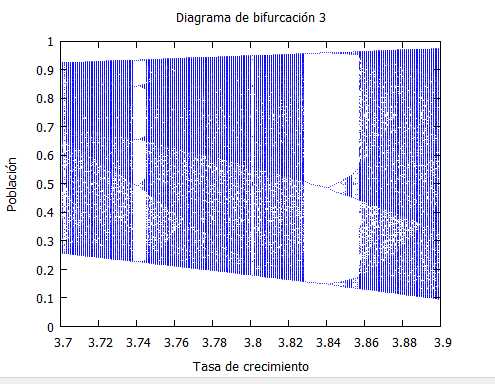
\includegraphics[width=.8\textwidth]{Imagen4.PNG}
\end{center}

Al acercarnos, comenzamos a ver la belleza del caos. Del ruido emergen extraños patrones y umbrales de turbulencias a cada lado del cual el sistema se comporta de manera muy diferente. Entre los parámetros de tasa de crecimiento de 3.82 y 3.84, el sistema pasa del caos nuevamente al orden, oscilando entre solo tres valores de población (aproximadamente 0.15, 0.55 y 0.95). Pero luego se bifurca nuevamente y vuelve al caos a tasas de crecimiento superiores a 3.86.

Se puede observar como se manifiestan algunos raros patrones y umbrales de turbulencias a cada lado del cual el sistema se comporta de manera muy diferente. Entre los parámetros de tasa de crecimiento de 3.82 y 3.84, el sistema pasa del caos  al orden, oscilando entre solo tres valores de población, sin embargo luego se bifurca nuevamente y vuelve al caos a tasas de crecimiento superiores a 3.86.

\subsection{Fractales y extraños atractores}

Acercándonos a los valores cercanos a 3.85:

\begin{center}
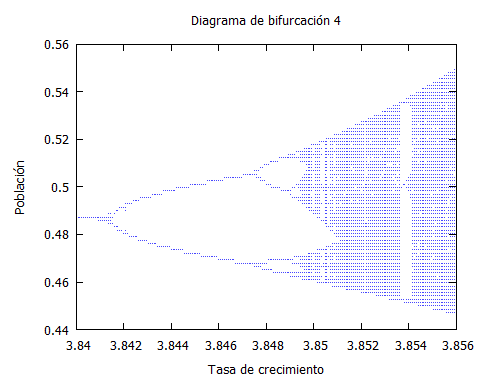
\includegraphics[width=.8\textwidth]{Imagen5.PNG}
\end{center}

Se puede ver la misma estructura exacta que vió en el nivel macro. En realidad, si se sigue haciendo zoom en este tramo, se seguirá viendo la misma estructura y patrones a escalas cada vez más finas, para siempre. Esto se debe a que los sistemas caóticos tienen atractores extraños y que su estructura se puede caracterizar como fractal . Los fractales son auto-similares, lo que significa que tienen la misma estructura en todas las escalas. Al acercarse a ellos, encontrará copias más pequeñas de la estructura más grande

Otra forma de visualizar esto es con un diagrama de fase (o diagrama de Poincaré ), que traza el valor de la población en la generación t + 1 en el eje  contra el valor de la población en t en el eje x.

Cómo el modelo sigue una regla determinista simple, si conocemos el valor poblacional de una determinada generación, podemos determinar el valor de la siguiente generación:

\begin{center}
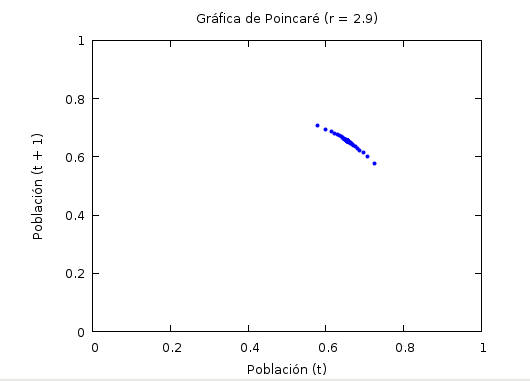
\includegraphics[width=.6\textwidth]{Imagen6.png}
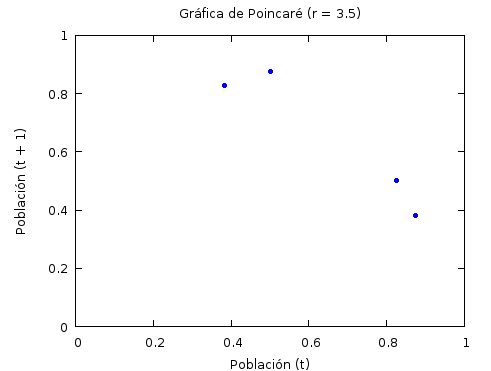
\includegraphics[width=.6\textwidth]{Imagen7.png}
\end{center}

El diagrama de fase de la izquierda modela como el mapa logístico se dirige hacia un atractor de punto fijo (en ambos ejes) cuando el parámetro de tasa de crecimiento se establece en 2.9. Cuando la tasa de crecimiento se establece en 3.5, el mapa logístico oscila en cuatro puntos, como se muestra la figura de la derecha. Esto corresponde a la porción verticar por encima de la tasa de crecimiento dada en los diagramas de bifurcación.

Esto es lo que sucede cuando estas bifurcaciones que duplican el período conducen al caos:

\begin{center}
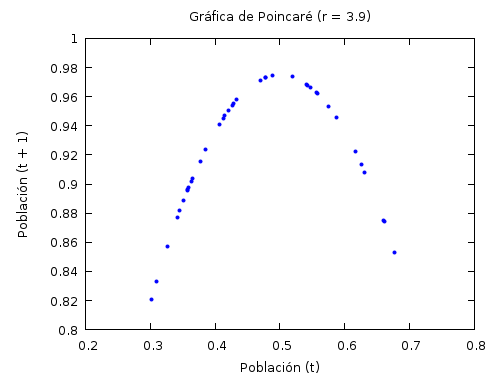
\includegraphics[width=.6\textwidth]{Imagen8.png}
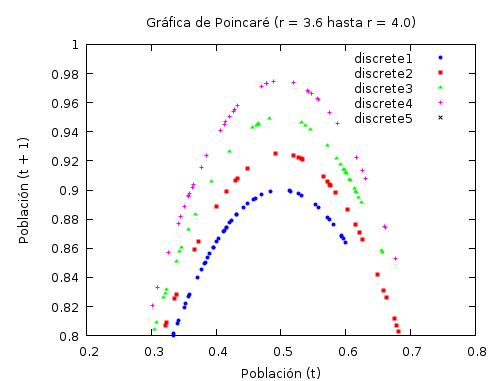
\includegraphics[width=.6\textwidth]{Imagen9.png}
\end{center}

Cada tasa de crecimiento forma su propia curva, debido a su geometría fractal y la naturaleza determinista de la ecuación logística estas parábolas nunca se superponen. La gráfica de la izquierda muestra una parábola formada por un valor de tasa de crecimiento. La gráfica de la derecha muestra 50 parámetros diferentes de tasa de crecimiento entre 3.6 y 4.0. Representando los valores de parámetros en los que el mapa logístico se comporta de manera caótica.

El sistema está extrañamente restringido, ya que nunca se asienta en un punto fijo o una oscilación constante. Simplemente rebota alrededor de diferentes valores de población, para siempre, sin repetir un valor dos veces, revelando extraños atractores.

\subsection{Caos vs aleatoriedad}

Los diagramas de fase son útiles para revelar atractores extraños en los datos de series de tiempo, porque insertan estos datos unidimensionales en un espacio de estado de 2 o incluso 3 dimensiones. Estos diagramas de fase representan un espacio imaginario que usa variables del sistema como sus dimensiones. Cada punto en el espacio de estado es un posible estado del sistema.

De hecho, puede ser difícil determinar si ciertas series de tiempo son caóticas o simplemente aleatorias cuando no se comprende por completo su dinámica oculta. Por ejemplo:

\begin{center}
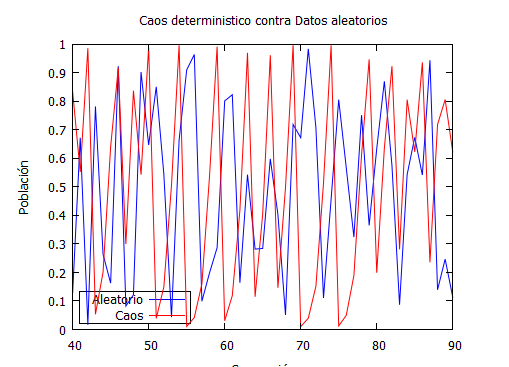
\includegraphics[width=.8\textwidth]{Imagen10.PNG}
\end{center}

Ambas líneas parecen saltar al azar, sin embargo, la línea azul representa datos aleatorios, pero la línea roja proviene del modelo logístico cuando la tasa de crecimiento se establece en 3.99. Este es un caos determinista, pero es difícil diferenciarlo de la aleatoriedad. Por lo tanto, se sugiere visualizar los dos conjuntos de datos con diagramas de fase:

\begin{center}
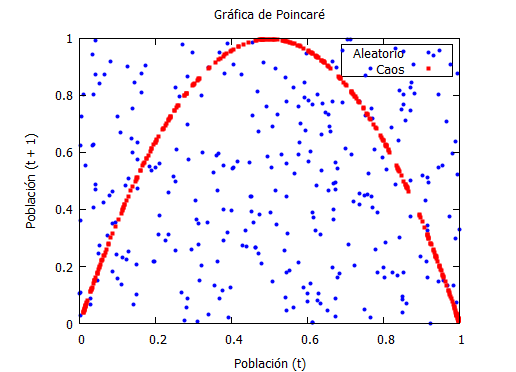
\includegraphics[width=.8\textwidth]{Imagen11.PNG}
\end{center}

Mientras, los datos aleatorios (en azul) solo parecen ruido, podemos ver el sistema caótico (en rojo) limitado por su atractor extraño. Esto es aún más convincente en el diagrama de fases 3-D que integra las series de tiempo en un espacio de estado tridimensional al representar el valor de la población en la generación t + 2 frente al valor en la generación t + 1 frente al valor en t .

En tres dimensiones , la estructura demuestra que los datos de series temporales aparentemente aleatorias del modelo logístico no son en absoluto aleatorios. En cambio, es un caos determinista aperiódico, limitado por un atractor extraño y alucinante.

\subsection{El efecto mariposa}

Los sistemas caóticos también se caracterizan por su dependencia sensible de las condiciones iniciales. A diferencia de un atractor de ciclo de punto fijo o límite, estos no tienen una cuenca de atracción que recolecte puntos cercanos a lo largo del tiempo. Por el contrario, con un atractor extraño, los puntos cercanos divergen con el tiempo.

Como se deben medir los parámetros y el estado del sistema con una precisión infinita, se dificultaba el modelado y la predicción del mundo real, ya que con la combinación de pequeños errores en la medición o el redondeo, el sistema se desconecta drásticamente. Fue a través de uno de esos errores de redondeo que Lorenz descubrió el caos por primera vez. Para mostrar esto, se ejecuta el modelo logístico con dos valores de población iniciales muy parecidos:

\begin{center}
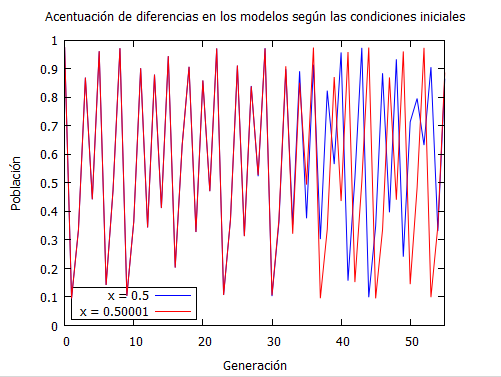
\includegraphics[width=.8\textwidth]{Imagen12.PNG}
\end{center}

Ambos tienen el mismo parámetro de tasa de crecimiento, sin embargo, la línea azul representa un valor poblacional inicial de 0.5 y la línea roja representa una población inicial de 0.50001. Siendo estas dos condiciones iniciales muy parecidas entre ellas. En consecuencia, sus resultados parecen esencialmente idénticos para las primeras 30 generaciones. Después de eso la diferencia en las condiciones iniciales comienza a complicarse. Para la generación 40, las dos líneas muestran poco en común.

Con el caos, la historia se pierde en el tiempo y la predicción del futuro es tan precisa como sus mediciones, mientras que en los sistemas caóticos del mundo real, las mediciones nunca son infinitamente precisas, por lo que los errores siempre se combinan, y el futuro se vuelve completamente desconocido desde tiempos suficientemente largos.

Esto es famoso por el efecto mariposa : una mariposa bate sus alas en China y provoca un tornado en Texas. Pequeños eventos compuestos e irreversiblemente alteran el futuro del universo.

\subsection{Las implicaciones del caos}

Los sistemas caóticos y fractales del mundo real incluyen grifos con fugas , helechos , frecuencias cardíacas y generadores de números aleatorios, es decir, pérdidas o escapes de información. Muchos estudiosos han estudiado las implicaciones de la teoría del caos para las ciencias sociales , las ciudades y la planificación urbana. Si embargo, como los efectos de las condiciones iniciales, aun que sean ligeramente distintas, se combinan con el tiempo, las intervenciones en un sistema pueden tener resultados impredecibles. Esto indica que existen límites para el conocimiento y la predicción. Causando como consecuencia que algunos futuros pueden ser desconocidos con precisión.

\section{Conclusión}

Me pareció un tema muy interesante, el cual considero que hubiera sido muy díficil de asimilar si no fuera por las gráficas que ayudan a aterrizar las ideas del autor. Fue de gran sorpresa poder realizar las gráficas, que en el artículo se generan con Phyton, en WxMaxima, ya que fue un gran salto entre lo que se había visto en la práctica anterior y ésta.

Ahora comprendó por que profesores de otros cursos nos recomendaban aprender a utilizar este tipo de softwares, ya que pueden ser de mucha ayuda para temas muy complejos.

\section{Bibliografía}

\begin{itemize}
\item Chaos Theory and the Logistic Map. (2015). Recuperado el 20 de mayo de 2018, de \url{http://geoffboeing.com/2015/03/chaos-theory-logistic-map/}
\item Chaotic dynamics with Maxima (2013). Recuperado el 20 de mayo de 2018, de \url{https://arxiv.org/pdf/1301.3240.pdf}
\item Aplicación Logística (2016). wikipedia.org. Recuperado el 20 de mayo de 2018, de \url{https://es.wikipedia.org/wiki/Aplicaci%C3%B3n_log%C3%ADstica}
\end{itemize}
\end{document}
